\section{Valley-Hall effect}
Up until now all of the various Hall effects we studied relied on a non-zero Chern number over the entire band. To do so, time symmetry breaking was needed.\\
The valley Hall effect is a particular kind of Hall effect that doesn't rely of time reversal breaking, however as explained in section \ref{sec:berry-symm} this means that to have a non zero Berry curvature, space inversion symmetry has to be broken. As explained in section \ref{sec:gapped-graphene} the inversion symmetry breaking can be achieved by resting the graphene sheet on top of a another honeycomb lattice that does not have sublattice symmetry like Molybdenum disulfide ($\textrm{MoS}_2$).\\
The problem with this approach is that no matter how strong the sublattice potential is, the Chern number of the valence and conduction band will always be zero.\\
However, if we treat the two valleys a two distinct quantum degrees of freedom, we have from equation \ref {eq:dirac-curvature-total} that for each of the valley equal and opposite non-zero Chern number.

\begin{equation}
    C=\pi\tau_z\,.
\end{equation}
This will lead to equal and opposite integer Hall conductivities in different Valleys. Now let's do more accurate calculations.

\subsubsection*{Calculation of the Hall conductivity as a function of the Fermi level}
In this section we are going to calculate the anomalous Hall conductivity for each valley as we change the chemical potential $\mu$ (or equivalently the Fermi level $E_\textrm{F}$). We can start by using the generalized TKNN formula \ref{eq:fermi-cond-2}, so the Hall conductivity $\sigma_{xy}$ is 
\begin{equation}
    \sigma_{xy}(\mu)=\tau_z\frac{e^2}\hbar \int_{\mathbb R^2} f[E^+(k)]\Omega^+_{k_xk_y}+f[E^-(k)]\Omega^-_{k_xk_y}\frac{d^2\vect k}{2\pi}\,,
    \label{eq:valley-conductivity-1}
\end{equation}
where $f(E)=\big[e^{\beta (E-\mu)}+1\big]^{-1}$ is the Fermi-Dirac distribution, it is applied once for the states with positive energy and once for the states with negative energy, and the $\pm$ sign represent the conduction band and the valence band quantum numbers ($\pm 1$).\\
We are going to analyze the system at low temperatures ($k_\beta T\ll 1$), so our Fermi-Dirac distribution can be considered like a step-function, for simplicity we are going to assume $\Delta>0$, if that is not true the resulting Hall conductivity will be reversed.\\
First let's integrate the conductivity for the conduction band.

\[
    \sigma^+_{xy}(\mu)=
    \frac{1}{(2\pi)^2}\frac {e^2}\hbar\int_{\mathbb R^2} f[E^+(k)]\Omega^+_{k_xk_y}dk_xdk_y=
    \frac{1}{(2\pi)^2}\frac {e^2}\hbar\int_{\mathbb R^2} f[E^+(q)]\Omega^+_{q_xq_y}dq_xdq_y\approx
\]

\[
    =\frac1{(2\pi)^2}\frac {e^2}\hbar \int_{\mathbb R^2}f[E^+(q)]\frac{\tau_z} 2\frac\Delta {E^3}dq_xdq_y
    \approx\frac{\Delta\tau_z}{2(2\pi)^2}\frac {e^2}\hbar
    \int_{0}^{2\pi}\int_{0}^{q_\textrm{F}} \frac{qdqd\theta}{E^3}=
\]

\[
    =\frac{\tau_z\Delta}{4\pi}\frac {e^2}\hbar
    \int_0^{q_f}\frac{qdq}{E^3} =\frac{\tau_z\Delta}{4\pi}\frac {e^2}\hbar\int_0^{q_f}\frac{qdq}{(\Delta^2+q^2)^{3/2}}= 
\]
\[
    =\frac{\tau_z\Delta}{4\pi}\frac {e^2}\hbar
    \left(\frac 1\Delta - \frac 1{\sqrt{\Delta^2+q_F^2}}\right)
    =\frac{\tau_z}2\frac{e^2}{2\pi\hbar}
    \left(
        1-\frac{\Delta}\mu
    \right)\theta(\mu-\Delta)\,.
\]
In the third passage we used equation \ref{eq:dirac-curvature-q} to express $\Omega_{q_xq_y}$, in the fourth passage we approximated the Fermi-Dirac to a step function.\\
The $\theta(\mu-\Delta)$ is there to make sure that if no states are inside the Fermi-Dirac the integral is zero.\\
So in the end we have that for the conduction band
\begin{equation}
    \sigma_{xy}^+(\mu)=
    \frac{\tau_z}2\frac{e^2}{2\pi\hbar}
    \left(
        1-\frac{\Delta}\mu
    \right)\theta(\mu-\Delta)\,.
\end{equation}
One thing to notice is that if you have $\mu \gg \Delta$ (aka. all states in the band are occupied) then the integral is equal to $-2\pi$. The integral of the lower band is very similar, the main difference is that the Berry curvature has opposite sign, and when integrating the Fermi-Dirac as a step function behaves like this:
\begin{equation}
\begin{split}
    \int_{\mathbb R^2}f[E^+(q)]dq_xdq_y&=
    2\pi\int_{0}^{q_\textrm{F}}dq\,,\\
    \int_{\mathbb R^2}f[E^-(q)]dq_xdq_y&=
    2\pi\int_{q_\textrm{F}}^\infty dq\,.
\end{split}
\end{equation}
In the end the conductivity contribution fro the valence band is
\begin{equation}
    \sigma_{xy}^-(\mu)=
    -\frac{\tau_z}2\frac{e^2}{2\pi\hbar}
        \frac{\Delta}\mu\theta(\Delta-\mu)\,.
\end{equation}
By the end equation of the conductivity for every $\mu$ is  \ref{eq:valley-conductivity-1} becomes
\begin{equation}
    \sigma_{xy}(\mu)=-\frac{\tau_z}2\frac {e^2}{2\pi \hbar}\Bigg[\frac{\Delta}{|\mu|}\theta\left(\mu^2-\Delta^2\right) + \theta\left(\Delta^2-\mu^2\right)\Bigg]\,.
    \label{eq:valley-conductivity-2}
\end{equation}

\begin{figure}[h]
    \centering
    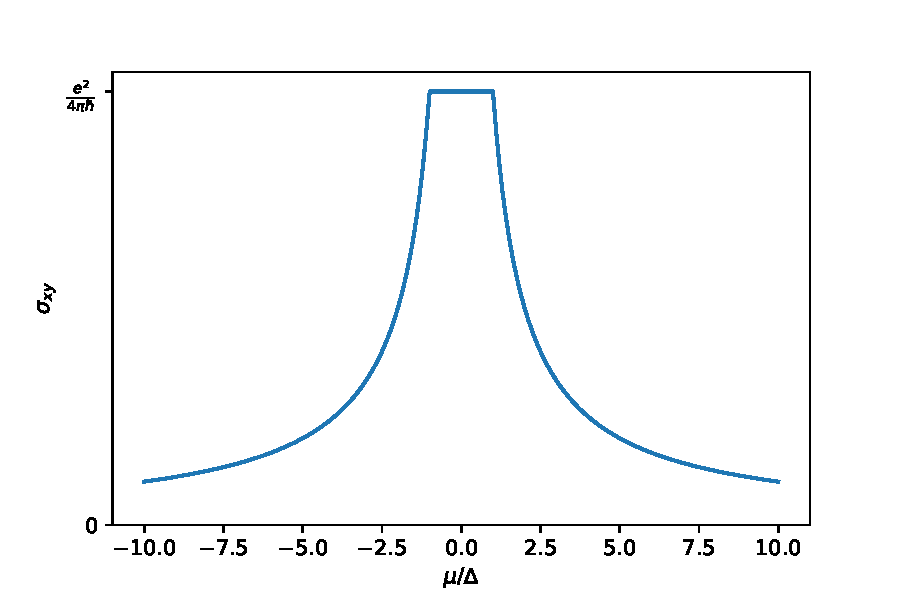
\includegraphics[width=\linewidth]{Immagini/ValleyHall/sigmaxy.pdf}
    \caption{Here is shown $\sigma_{xy}(\mu)$ (eq. \ref{eq:valley-conductivity-2}). Notice how, when $\mu \in [-\Delta,\Delta]$ then $\sigma_{xy}=\frac {e^2}{4\pi \hbar}$}
    \label{fig:sigma_xy}
\end{figure}


However in most cases it's safe to assume that the chemical potential is inside the energy gap, so equation \ref{eq:valley-conductivity-2} becomes
\begin{equation}
    \sigma_{xy}=\frac{\tau_z}2\frac {e^2}{2\pi \hbar}\,.
\end{equation}


\section{Topological properties of bilayer graphene}

As explained in section \ref{sec:bilayer} the Hamiltonian for the low energy states bilayer graphene is (equation \ref{eq:bilayer_ham})
\begin{equation}
\begin{split}
    H=&H_2+h_w+h_4+h_\Delta+h_U+h_{AB}\,,\\
    H_2=&-\frac1 {2m}\begin{bmatrix}
        0 & (\pi^\dag)^2\\
        \pi^2 &0\\
    \end{bmatrix}\,,
\end{split}
\end{equation}
where $H_2$ is the dominant term and the others are perturbations.
For a given momentum $\vect p=[p\cos\phi,p\sin\phi]$ a Hamiltonian $H_J$ can be written in the form
\begin{equation}
    H_J=E(p)\vect n(\phi)\cdot \vect \sigma\,,
\end{equation}
where $\vect n(\phi)=-[\cos(J\phi),\sin(J\phi)]$ and $\vect \sigma$ is the vector made of Pauli matrices. For bilayer graphene $J=2$ while for monolayer $J=1$, this convention of using $J$ thus helps us compare what happens between the two cases.
The eigenstates in both cases are (equations \ref{eq:monolayer_eigenstates} and \ref{eq:bilayer_eigenstates})
 \begin{equation}
    \ket{\pm,\vect k}=
    \frac 1{\sqrt 2}
    \begin{bmatrix}
        1\\
        \mp e^{i2\phi}
    \end{bmatrix}
    e^{i\vect k\cdot \vect r}\,,\quad
    \vect k=kn(\phi)\,.
\end{equation}
The eigenstates of $H_J$ correspond to pseudospins polarized parallel (electrons) or antiparallel (holes) to the ‘quantization’ axis $\vect n$. An adiabatic evolution of such pseudospin states, which accompanies the rotation of momentum $\vect k$ by angle $\phi$, also corresponds to the rotation of axis $\vect n$ by angle $J\phi$.\\
As a result, if a electron encircles a closed contour in the momentum space (that is $\phi = 2\pi$), a phase shift $\Phi = J \pi$ known as Berry’s phase is gained by the quasiparticle’s wavefunction.\\
As a result the Chern number on each Dirac cone in bilayer graphene is double the one of single layer graphene, this means that the Hall effect is doubled in bilayer graphene.

\section{Non-local Charge transport}
\label{sec:beconcini}
If we apply a voltage $V$ in two opposite points of a strip of a ohmic material of width $W$ and infinite lenght, and  we see a current that flows from one point to another figure \ref{fig:beconcini_strip}.\\
\begin{figure}[h]
    \centering
    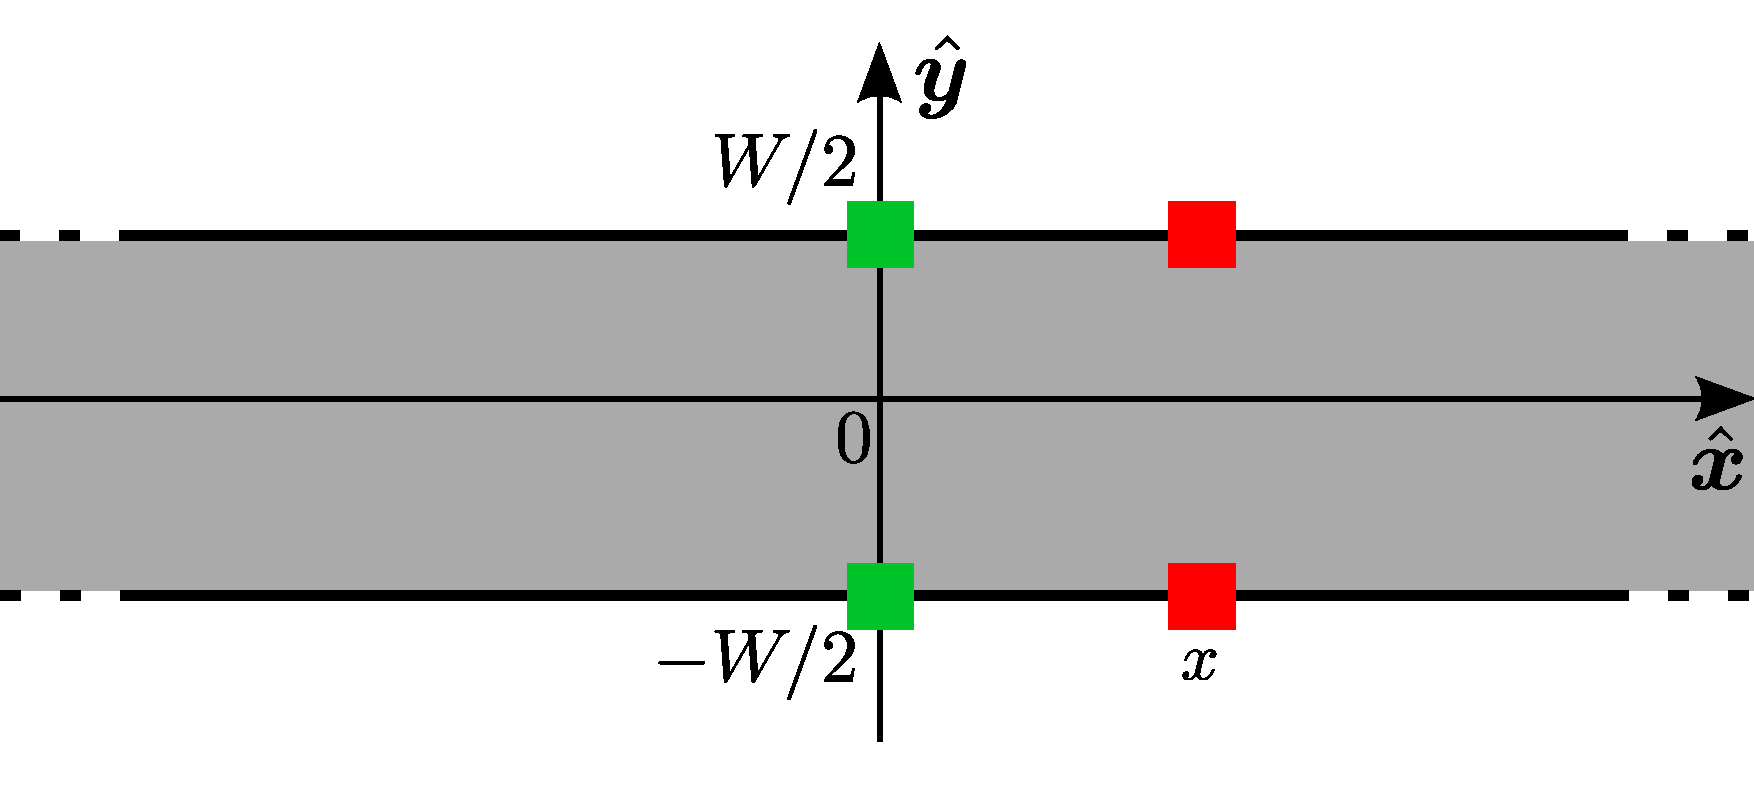
\includegraphics[width=0.7\linewidth]{Immagini/ValleyHall/beconcini_strip.pdf}
    \caption{Representation of the strip. The current goes from one of the green squares in the middle to the other, while the voltage is measured from the two red squares on the right. Image taken from \cite{Beconcini_2016}}
    \label{fig:beconcini_strip}
\end{figure}
Clearly the current isn't completely localized along the axis that unites the two injection points, and so does the voltage difference.\newline
If we probe the voltage from two different points with an offset of $x$ from the injection points and we divide it by the total current between the contacts we see that  

\begin{equation}
    \frac{V(x)}I=\frac{2\rho}\pi\ln\bigg |\coth \Big(\frac{\pi x}{2W}\Big)\bigg |\,,
    \label{eq:ohmic signal}
\end{equation}
where $\rho$ is the resistivity. We will later give a proof for this formula.

Two-dimensional material like gapped graphene \cite{gorbachev2014detecting,sui2015gate,shimazaki2015generation} and transition metal dichalcogenides \cite{xiao2012coupled,mak2014valley,lee2017valley}, do not obey this equation. This is because these materials display the Valley Hall effect we talked about previously.

Non-local transport can be a useful tool to probe the existence of anomalous Hall effect \cite{valenzuela2006direct,abanin2009nonlocal,brune2010evidence,abanin2011giant,balakrishnan2013g,wang2015proximity}


\section{Theory of non local charge transport}

The charges inside the material get pushed around from the electrochemical potential $\psi_K$


\begin{equation}
    \psi_{K}(\vect r)= V(\vect r)-\frac 1e \mu_K[n_{K_1}(\vect r),n_{K_2}(\vect r),T]\,,
\end{equation}
where $\phi$ is the electrical potential, and $\mu_K=\frac {\partial}{\partial n_{K}}F[n_{K_1}(\vect r),n_{K_2}(\vect r),T]$ is the chemical potential of the material and $F$ is the free energy.

The current generated from this potential in the valley $K_\alpha$ in the $i-$th direction is

\begin{equation}
    -eJ_{K_\alpha,i}(\vect r)= \sum_{j,b} \underbrace{-\sigma_{K_\alpha K_\beta ,ij}}_{\textrm{conductivity}}\partial_j\psi_{K_\beta }(\vect r)\,.
\end{equation}
From now we are going to set $T\approx 0$\footnote{A more precise statement is that the thermal De Broglie wavelenght $\lambda_T$ must be much larger than the average distance between the electrons. We are not going into the math here, but if you want to calculate it, keep in mind that the dispersion relation is relativistic, so the formula of $\lambda_T$ is going to be a bit different}
and ignore intervalley scattering, so if $K_\alpha \neq K_\beta $ $\sigma_{K_\alpha K_\beta ,ij}=0$, also because of this the free energy can be written as the sum of the two Free energies
\begin{equation}
    F(n_{K_1},n_{K_2})=F_1(n_{K_1}(\mathbf r))+F_2(n_{K_2}(\mathbf r))\,,
\end{equation}
and so the chemical potential of a given valley depend only on the number of electron in the same valley
\begin{equation}
    \mu_\alpha(n_{K_\alpha}(\mathbf r))=\frac{\partial}{\partial n_{K_\alpha}}F(n_{K_0},n_{K_1})=\frac{\partial}{\partial n_{K_\alpha}}F_\alpha(n_{K_\alpha}(\mathbf r))\,.
\end{equation}
This simplifies the trasport equation in 

\begin{equation}
    -e\mathbf J_{K_{\alpha}}(\mathbf r)= \sigma_{K_\alpha}(\mathbf r)\nabla \psi_{K_\alpha}(\mathbf r)\,.
    \label{eq:current-1}
\end{equation}
Where $\sigma_{K_\alpha}$ is the following matrix
\[
    \sigma_{K_\alpha}=
    \begin{bmatrix}
        \sigma_{K_\alpha K_\alpha,xx} & \sigma_{K_\alpha K_\alpha,xy}\\
        -\sigma_{K_\alpha K_\alpha,xy}^* & \sigma_{K_\alpha K_\alpha,xx}
    \end{bmatrix}\,.
\]
Now we need to write the gradient electrochemical potential $\nabla \psi(\vect r)$
\begin{equation}
    \nabla \psi_{K_\alpha}(\mathbf r)=\nabla V(\mathbf r) -\frac 1e \frac{\partial}{\partial n_{K_\alpha}}\mu_\alpha(n_{K_\alpha}(\mathbf r))\nabla n_{K_\alpha}\,.
    \label{eq:echemical1}
\end{equation}
For gapped Dirac Hamiltonians

\[
\frac{\partial \mu_{K_\alpha}}{\partial n_{K_\alpha}}=\frac{\pi}{\sqrt{2\pi |n|+\Delta^2}}+\Delta\delta(n)\approx \frac \pi\Delta +\Delta\delta(n) \quad \forall \alpha\,.
\]
In this equation we assumed that there are very few charge carries, so $\frac n{\Delta^2}\approx 0$. We can shorten the equation \ref{eq:echemical1} by defining
\begin{equation}
    e^2D_{K_\alpha,ij}=\sigma_{K_\alpha, ij}\frac{\partial \mu_\alpha}{\partial n_{K_\alpha}}[n_{K_\alpha}(\mathbf r)]\,,
\end{equation}
so equation \ref{eq:current-1} becomes

\begin{equation}
    -eJ_{K_\alpha,i}(\mathbf r)=\sigma_{K_\alpha, ij}E_j(\mathbf r) -eD_{K_\alpha,ij}\partial _jn_{K_\alpha}(\mathbf r)\,,
\end{equation}
or, written in matrix form
\begin{equation}
    -e\mathbf J_{K_\alpha}(\mathbf r)=\sigma_{K_\alpha}\mathbf E(\mathbf r) -eD_{K_\alpha}\nabla n_{K_\alpha}(\mathbf r)\,,
\end{equation}
where $\sigma_{K_\alpha}$ and  $-eD_{K_\alpha}$ are matrices.

\subsection{Re-writing the equations in terms of charge current and valley current}
Measuring the currents in different valley can be cumbersome, however measuring the charge current $\mathbf J_{c}=\mathbf J_{K_1}+\mathbf J_{K_2}$ is straightforward, and for mathematical convenience we also define the valley current $\mathbf J_{v}=\mathbf J_{K_1}-\mathbf J_{K_2}$.

Since we no longer describe the currents in terms of their valley index, but on the sum and the difference of what happens at the different valleys, we are going to reparametrize also the other quantities in the same fashion.


\begin{equation}
    \begin{cases}
        \sigma_c=\sigma_{K_1}+\sigma_{K_2}=2\sigma_{xx}\delta_{ij}\\
        \sigma_v=\sigma_{K_1}-\sigma_{K_2}=\sigma_v=2\sigma_{xy}\epsilon_{ij}
    \end{cases}\,.
\end{equation}
The term $-eD_{K_\alpha}\nabla n_{K_\alpha}(\mathbf r)$ is a little harder to translate. First off we are going to impose the local charge conservation

\[
    n(\mathbf r)=n_{K_0}+n_{K_1}\approx 0\,,
\]
and so 

\begin{equation}
    n_v(\mathbf r)=n_{K_1}-n_{K_2}=2n_{K_1}=-2n_{K_2}\,.
\end{equation}
Now let's do the sum of the $D_{K_\alpha}\nabla n_{K_\alpha}(\mathbf r)$ terms to write them in terms of charge and valleys degrees of freedom

\[
    D_{K_1}\nabla n_{K_1}+D_{K_2}\nabla n_{K_2}=(D_{K_1}-D_{K_2})\nabla n_v(\mathbf r)/2\,,
\]

\[D_{K_1}-D_{K_2}=\sigma \frac{\partial \mu_1}{\partial n_{K_1}}- \sigma^T \frac{\partial \mu_2}{\partial n_{K_2}}\,.\]
Since $\mu_v=2\mu_1=-2\mu_2$ and $n_v=2n_{K_1}=-2n_{K_2}$

\[D_{K_1}-D_{K_2}=\frac 1{e^2}(\sigma-\sigma^T)\frac{\partial \mu_v}{\partial n_v}=\frac 2{e^2}\sigma_v\frac{\partial \mu_v}{\partial n_v}\,.\]
So I define 

\[D_{cv}=\frac 2{e^2}\sigma_v\frac{\partial \mu_v}{\partial n_v}\approx\frac 2{e^2} \frac \pi\Delta\sigma_v\,,\]
and we get that

\[D_{K_1}\nabla n_{K_1}+D_{K_2}\nabla n_{K_2}=D_{cv}n_v\,.\]
Putting it all together we have that

\[\mathbf J_c(\mathbf r)=\sigma_c \mathbf E(\mathbf r)+eD_{cv}\nabla n_v(\mathbf r)\,.\]
Writing all the indices

\begin{equation}
    J_{c,i}(\vect r)=\sum_j \sigma_{c,xx}\delta_{ij}E_i(\vect r)+eD_{cv,xy}\epsilon_{ij}\partial_j n_v(\vect r)\,,
\end{equation}
so we can rewrite them as


\begin{equation}
    \mathbf J_{c}= \sigma_{c,xx}\mathbf E_i + D_{cv,xy} \nabla \times n_v\,,
    \label{eq:diff-jc}
\end{equation}
where $\sigma_{c,xx}$ and $D_{cv,xy}$ are scalars.

And now the difference of the $D_{K_\alpha}\nabla n_{K_\alpha}(\mathbf r)$ terms to write them in terms of charge and valleys degrees of freedom

\[D_{K_0}\nabla n_{K_0}-D_{K_1}\nabla n_{K_1}=(D_{K_0}+D_{K_1})\nabla n_v(\mathbf r)/2\,,\]
and with some calculations done in a similar fashion to the one we use to calculate $\mathbf J_c$ we have that

\[D_v=\frac12(D_{K_0}+D_{K_1})=\frac 1{e^2}\sigma_c\frac{\partial \mu_c}{\partial n_c\,,}\]
so, in matrix form


\begin{equation}
    \mathbf J_v(\mathbf r)=\sigma_v\mathbf E(\mathbf r)+eD_{v}\nabla n_v(\mathbf r) \,,   
\end{equation}
which can be re-written as


\begin{equation}
    J_{v,i}(\mathbf r)=\sum_j \sigma_{c,xy} \epsilon_{ij}  E_j(\mathbf r)+eD_{v,xx}\delta_{ij}\partial_j n_v(\mathbf r)
    \,,
    \label{eq:diff-jv}  
\end{equation}
where $\sigma_{c,xy}$ and $D_{v,xx}$ are scalars.


\subsection{Laplace equation}

Now that we have the charge and valley currents differential equations we calculate the laplacians to solve them. Let's start from the equation for the charge currents \ref{eq:diff-jc}

\begin{equation}
    \nabla \cdot \vect J_c=\nabla \cdot (\sigma_c \mathbf E)+ eD_{cv,xx}\nabla \cdot (\nabla\times n_v)\,.
    \label{eq:lap-jc}
\end{equation}
Inside the material the are no sources of charge current, so $\nabla \cdot \vect J_c=$, and the divergence of a rotor is zero, so $\nabla \cdot (\nabla\times n_v)=0$. This means that inside the material
\begin{equation}
    \boxed{
    \nabla^2 V(x,y)=0
    }
\end{equation}
So, to be able to solve the laplace equation we just need to impose the boundary conditions that the current is injected in a single point at $x=0$ along the $\hat{\vect y}$ direction. 
\[
    -e\vect J_c(x,\pm W/2)=I\delta(x)\hat{\vect y}\,.
\]
If we put it in equation \ref{eq:lap-jc} we get
\begin{equation}
    \boxed{
        I\delta(x)=\sigma_{c,xx}\partial_y V(x,\pm W/2)-eD_{cv,xy}\partial_x n_v(x,\pm W/2)
    }
\end{equation}
Now let's calculate the laplacian for the valley current equation \ref{eq:diff-jv}


\begin{equation}
    \nabla \cdot \mathbf J_v=\nabla \times (\sigma_{c,xy} \mathbf E)+ e\nabla \cdot (D_{v,xx}\nabla n_v)\,.
\end{equation}
Now, lets analyze all the terms one by one
\begin{itemize}
\item For the continuity equation we have that $\nabla \cdot \mathbf J_v=\frac \partial {\partial t} n_v$, since intervalley scattering is zero, this should be zero, however we can reintroduce it by adding a exponential decay for the valley imbalance of charges $\frac \partial {\partial t} n_v=-\frac 1 {\tau_v} n_v$
\item$e\nabla \cdot (D_{v,xx}\nabla n_v)$ is really nothing special, inside the material $D_{v,xx}$ is constsant so in the end it is equal to $eD_{v,xx}\nabla^2 n_v$
\item $\nabla \times (\sigma_{c,xy} \mathbf E)$ is equal to zero inside the material, but on the edge can be non-zero because $\sigma_{c,xy}$ changes form inside to the outside
\end{itemize}
In the end we get that


\begin{equation}
    eD_{v,xx}\nabla^2n_v=-\frac 1{\tau_v}n_v- \nabla \times (\sigma_{c,xy} \mathbf E)\,.
\end{equation}
This means that at the equilibrium $n_v\neq 0$ only if you are were $\nabla\times (\sigma_{c,xy} \mathbf E)\neq 0$, and this is only true along the edge, so we we'll have to worry about this term only in the boundary conditions, So

\begin{equation}
    \boxed{\bigg[
        \nabla^2 -\frac 1{\tau_v D_{v,xx}}
        \bigg]
    n_v(\vect r)=0}
\end{equation}
The boundary condition is simply that the valley current doesn't exit the material, so
\begin{equation}
    J_{v,y}(x,\pm W/2)=0\,.
\end{equation}
Putting it into the differential equation for $J_v$ (eq \ref{eq:diff-jv}) we get
\begin{equation}
    \boxed{
        \sigma_{v,xy}\partial_x V(x,\pm W/2)+eD_{v,xx}\partial_y n_v(x,\pm W/2)=0
    }
\end{equation}


All the boxed equations we wrote in the in this section enable us to completely solve the system. For convenience let's write the m in a single system of equations

\begin{equation}
    \begin{cases}
        \nabla^2 V(x,y)=0\\
        \bigg[\nabla^2 -\frac 1{\tau_v D_{v,xx}}\bigg]n_v(\vect r)=0\\
        I\delta(x)=\sigma_{c,xx}\partial_y V(x,\pm W/2)-eD_{cv,xy}\partial_x n_v(x,\pm W/2)\\
        \sigma_{v,xy}\partial_x V(x,\pm W/2)+eD_{v,xx}\partial_y n_v(x,\pm W/2)=0
    \end{cases}\,.
    \label{eq:syst1}
\end{equation}
From the third equation in the system above we can see that $V(x,y)$ is even along the $\hat{\vect x}$ axis and odd along the $\hat{\vect y}$ axis.\newline
From the fourth equation we can see that $n_v$ has the opposite parity to $V$, so it's odd along the $\hat{\vect x}$ axis and even along the $\hat{\vect y}$ axis.\newline

To be able to solve it we first have to do a Fourier transform over the $\hat{\vect x}$ direction. The first two equations of eq \ref{eq:syst1} becomes


\begin{equation}
    \begin{cases}
        (\partial_y^2 - k^2) V(k,y)=0\\
        \big[\partial_y^2 -\omega^2(k)\big]n_v(k,y)=0
    \end{cases}\,.
\end{equation}
The solutions that respect the symmetries we talked about earlier are
\begin{equation}
    V(k,y)=V(k)\sinh (ky)\,; \quad \quad n_v(k,y)=n_v(k)\cosh [\omega(k)y]\,.
    \label{eq:separation}
\end{equation}
However we still do not know what are $V(k)$ and $n_v(k)$, to obtain them we have to plug the equations above in the last two equations of \ref{eq:syst1}
\begin{equation}
    \begin{cases}
        \sigma_{c,xx}k\cosh(kw/2) V(k)-eD_{cv,xy}ik \cosh(\omega W/2)n_v(k)=I\\
        -\sigma_{v,xy} ik \sinh(kw/2) V(k)-eD_{v,xx}\omega(k)\sinh(\omega W/2) n_v(k)=0
    \end{cases}\,.
\end{equation}
This system of equation is linear in $V(k)$ and $n_v(k)$, so it can be written in this form
\begin{equation}
    \begin{bmatrix}
        A&B\\
        C&D
    \end{bmatrix}
    \begin{bmatrix}
        V\\n_v
    \end{bmatrix}=
    \begin{bmatrix}
        I\\0
    \end{bmatrix}\,.
\end{equation}
And the inverse is simply
\begin{equation}
    \begin{bmatrix}
        V\\n_v
    \end{bmatrix}=
    \frac I{AD-BC}
    \begin{bmatrix}
        D\\-C
    \end{bmatrix}\,.
\end{equation}
Since we want only care to calculate the voltage we only need to evaluate
\[
    V=\frac{I}{A-\frac{BC}D}    \,,
\]
wich turns out to be equal to
\begin{equation}
    V(k)=\frac I{\sigma_c}\frac{\omega(k)/k}{\sinh(kW/2)}
    \bigg\{
        \frac{\omega(k)}{\tanh(kW/2)} + \frac{k\tan^2(\theta_{VH})}{\tanh[\omega(k)W/2]}    
    \bigg\}^{-1}\,.
    \label{eq:vk}
\end{equation}
We can plug it into equation \ref{eq:separation} and evaluate it at $y=\pm W/2$

\begin{equation}
    V(k,\pm W/2)=V(k)\sinh(\pm kW/2)=\frac{I\omega}{\sigma_c k}\bigg\{\dots\bigg\}^{-1}\,,
\end{equation}
where the terms inside the curly brakets are the same from the previous equation (\ref{eq:vk}).\\
Finally we can calculate the non-local resistance

\begin{equation}
    R_\textrm{NL}(k)=\frac{V(k,W/2)-V(k,-W/2)}I\,,
\end{equation}
which is equal to

\begin{equation}
    R_\textrm{NL}(k)=\frac{2\omega(k)}{k\sigma_c}
    \bigg\{
        \frac{\omega(k)}{\tanh(kW/2)} + \frac{k\tan^2(\theta_{VH})}{\tanh[\omega(k)W/2]}    
    \bigg\}^{-1}\,.
   \label{eq:fre-response-beconcini}
\end{equation}
Understanding this formula will enable us to fully model how electrons behave in Hall bars, and the study of this formula will be the main focus of the last chapter.


